\documentclass[aspectratio=169,10pt]{beamer}

\usetheme{Madrid}
\usecolortheme{default}
\setbeamertemplate{navigation symbols}{}
\setbeamertemplate{footline}[frame number]

\usepackage{graphicx}
\usepackage{booktabs}
\usepackage{amsmath}
\usepackage{hyperref}

% University of Minnesota colors
\definecolor{umnmaroon}{RGB}{122,0,25}
\definecolor{umngold}{RGB}{255,204,51}
\definecolor{umnlightgold}{RGB}{255,229,153}

% Apply color theme
\setbeamercolor{structure}{fg=umnmaroon}
\setbeamercolor{palette primary}{bg=umnmaroon,fg=white}
\setbeamercolor{palette secondary}{bg=umnmaroon,fg=white}
\setbeamercolor{palette tertiary}{bg=umngold,fg=umnmaroon}
\setbeamercolor{palette quaternary}{bg=umnmaroon!90,fg=white}
\setbeamercolor{titlelike}{parent=palette primary}
\setbeamercolor{frametitle}{bg=umnmaroon,fg=umngold}
\setbeamercolor{block title}{bg=umnmaroon,fg=umngold}
\setbeamercolor{block body}{bg=umnmaroon!10,fg=black}
\setbeamercolor{block title example}{bg=umngold,fg=umnmaroon}
\setbeamercolor{block body example}{bg=umngold!20,fg=black}


% Navigation symbols in maroonontrolled, sustained arm c
\setbeamercolor{section in head/foot}{bg=umnmaroon,fg=umngold}
\setbeamercolor{subsection in head/foot}{bg=umnmaroon!75,fg=white}


\graphicspath{{../images/}{../images/Results/}}

\title{Tailorable Force-Sensing Skins for Manipulators Using Textile and Additive Manufacturing}
\subtitle{IROS 2026 Submission}
\author{Adam Imdieke, Heidi Woelfle, Brad Holschuh and Karthik Desingh}

\date{}

\begin{document}

\begin{frame}
    \titlepage
\end{frame}

\begin{frame}{Why Whole-Arm Force Sensing?}
    \begin{columns}[T]
        \begin{column}{0.42\textwidth}
            \footnotesize
            \begin{itemize}
                \item Contact occurs along the arm, not only at the gripper.
                \item Mobile manipulation needs:
                \begin{itemize}
                    \item low-force contact avoidance,
                    \item high-force contact embracing.
                \end{itemize}
                \item Goal: low-cost, high-coverage, deployable skins.
            \end{itemize}
        \end{column}
        \begin{column}{0.58\textwidth}
            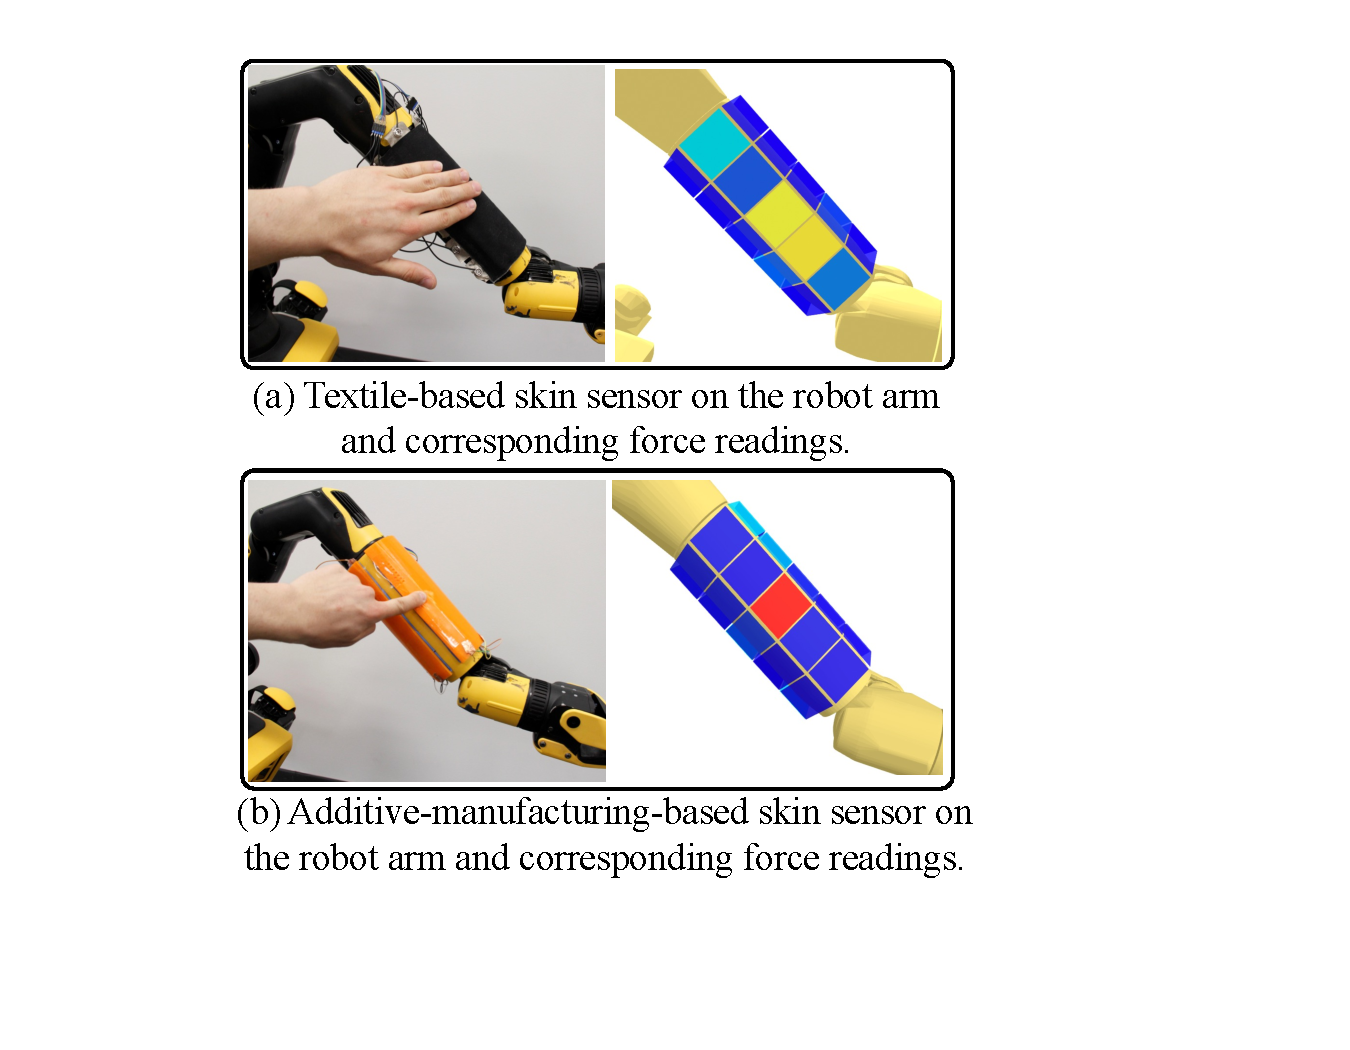
\includegraphics[width=\linewidth,height=0.72\textheight,keepaspectratio]{Teaser_both_v6.pdf}
        \end{column}
    \end{columns}
\end{frame}

\begin{frame}{Approach: Two Complementary Sensor Architectures}
    \centering
    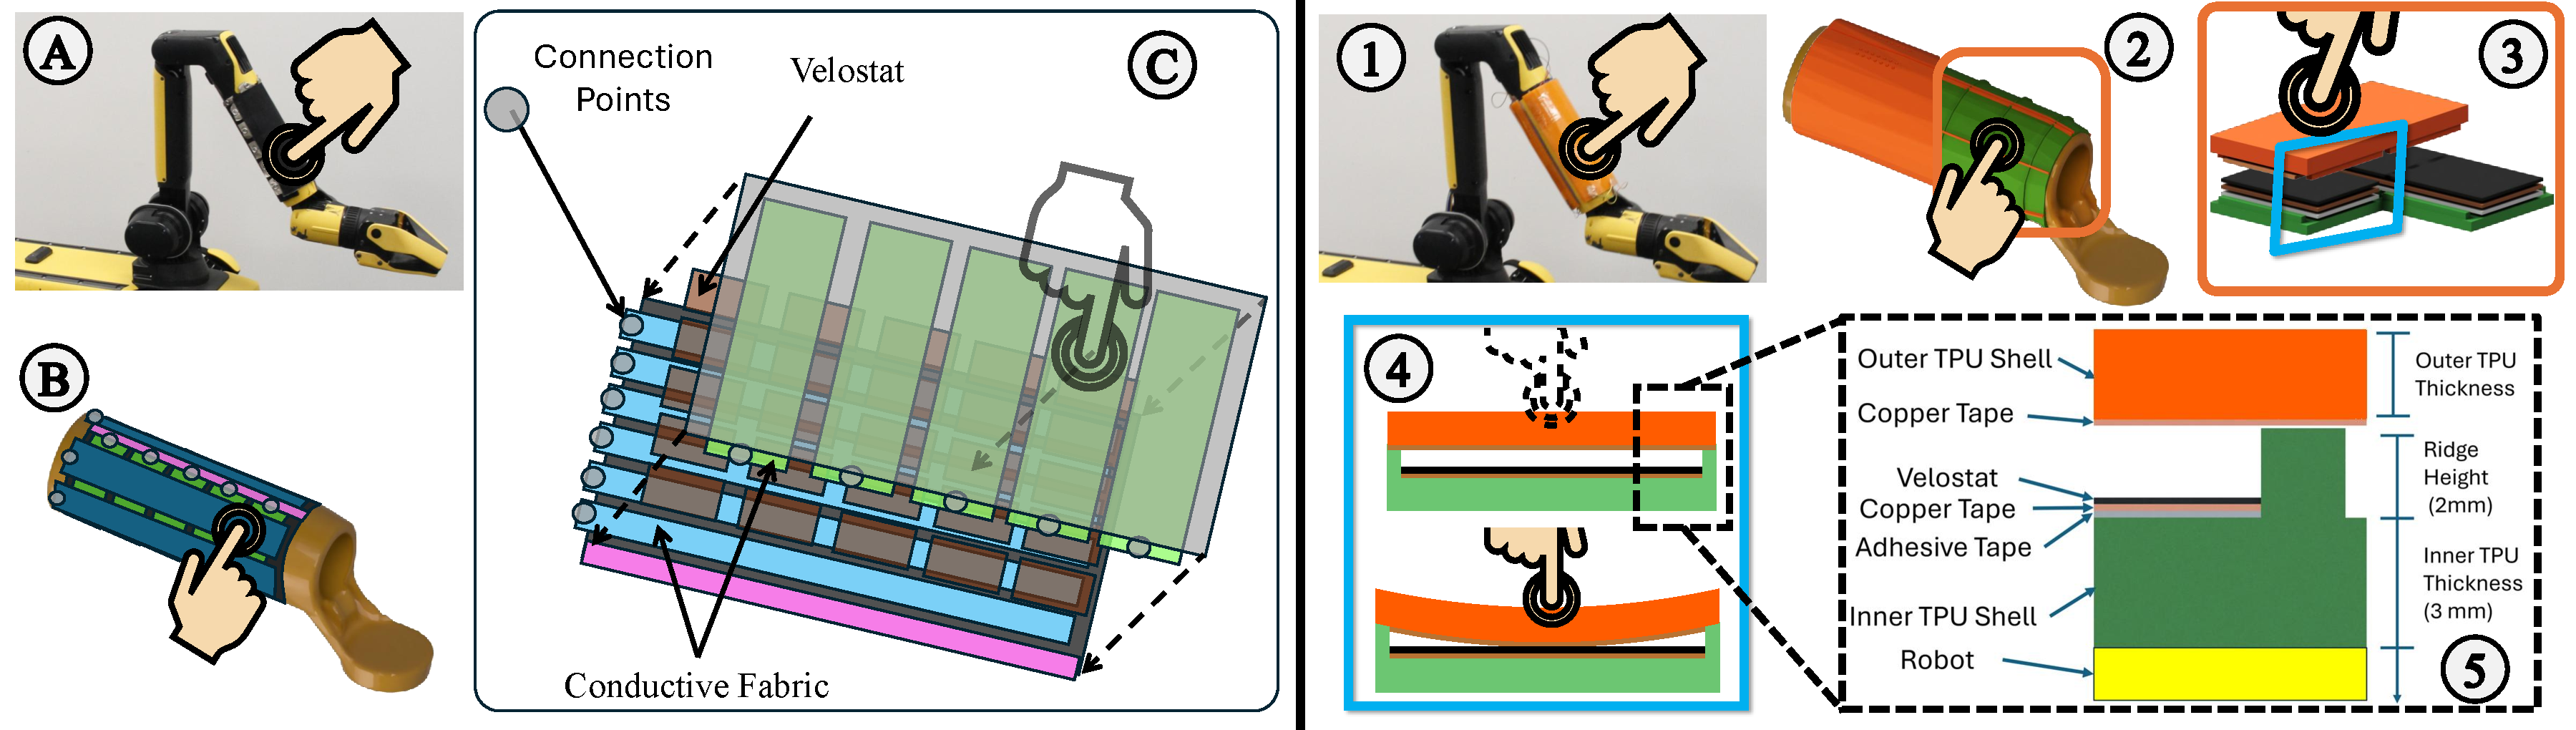
\includegraphics[width=0.92\linewidth]{Sensor_Overall_Both_v4.pdf}

    \vspace{0.5em}
    \small
    Textile skin: high sensitivity and flexibility.\hfill
    AM skin: conformal, higher-force operation.
\end{frame}

\begin{frame}{Electronics and Force Modeling}
    \begin{columns}[T]
        \begin{column}{0.50\textwidth}
            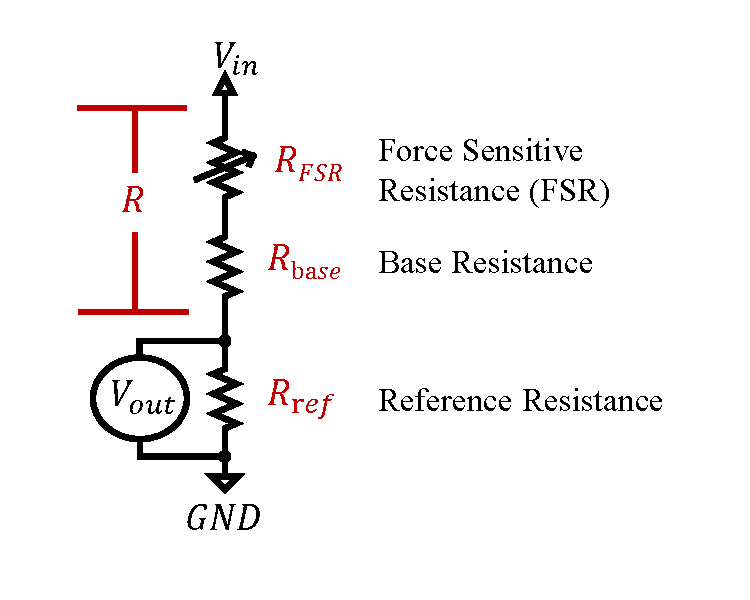
\includegraphics[width=\linewidth]{Circuit_v2.pdf}
        \end{column}
        \begin{column}{0.50\textwidth}
            \small
            Taxels are read with a voltage divider, then mapped to force via:
            \[
                R(F)=A F^B + R_{\mathrm{base}},
                \quad
                F=\left(\frac{R-R_{\mathrm{base}}}{A}\right)^{1/B}
            \]
            \vspace{0.4em}
            \begin{itemize}
                \item Per-taxel calibration from load/unload data.
                \item Shared framework for both sensor families.
            \end{itemize}
        \end{column}
    \end{columns}
\end{frame}

\begin{frame}{Main Characterization Result}
    \centering
    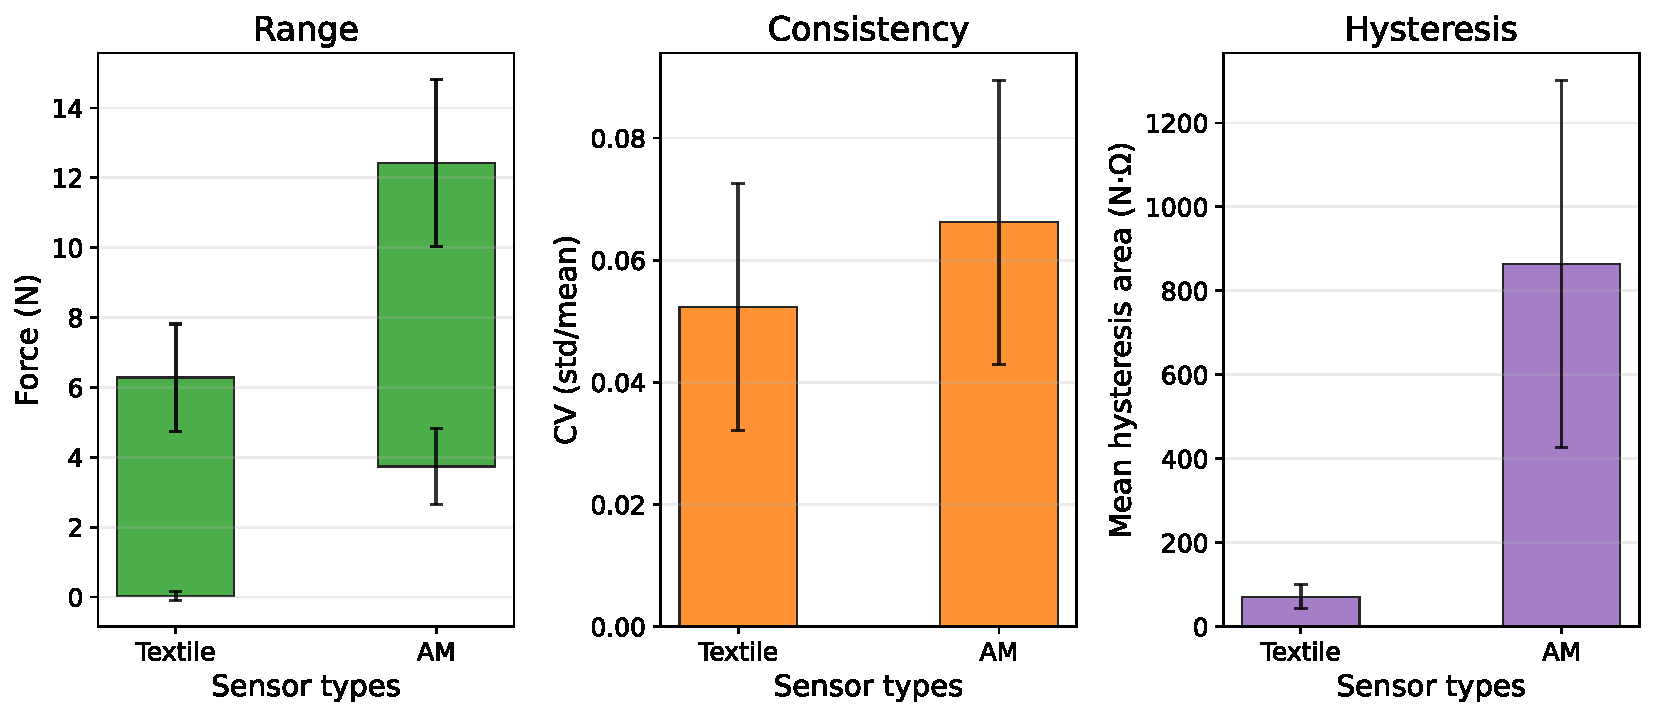
\includegraphics[width=0.95\linewidth,height=0.70\textheight,keepaspectratio]{overall_range_repeatability_hysteresis.pdf}

    \vspace{0.4em}
    \small
    Textile: lower-force sensitivity and low hysteresis.\hfill
    AM: higher-force operation but less repeatable.
\end{frame}

\begin{frame}{Real-World Validation on Spot}
    \centering
    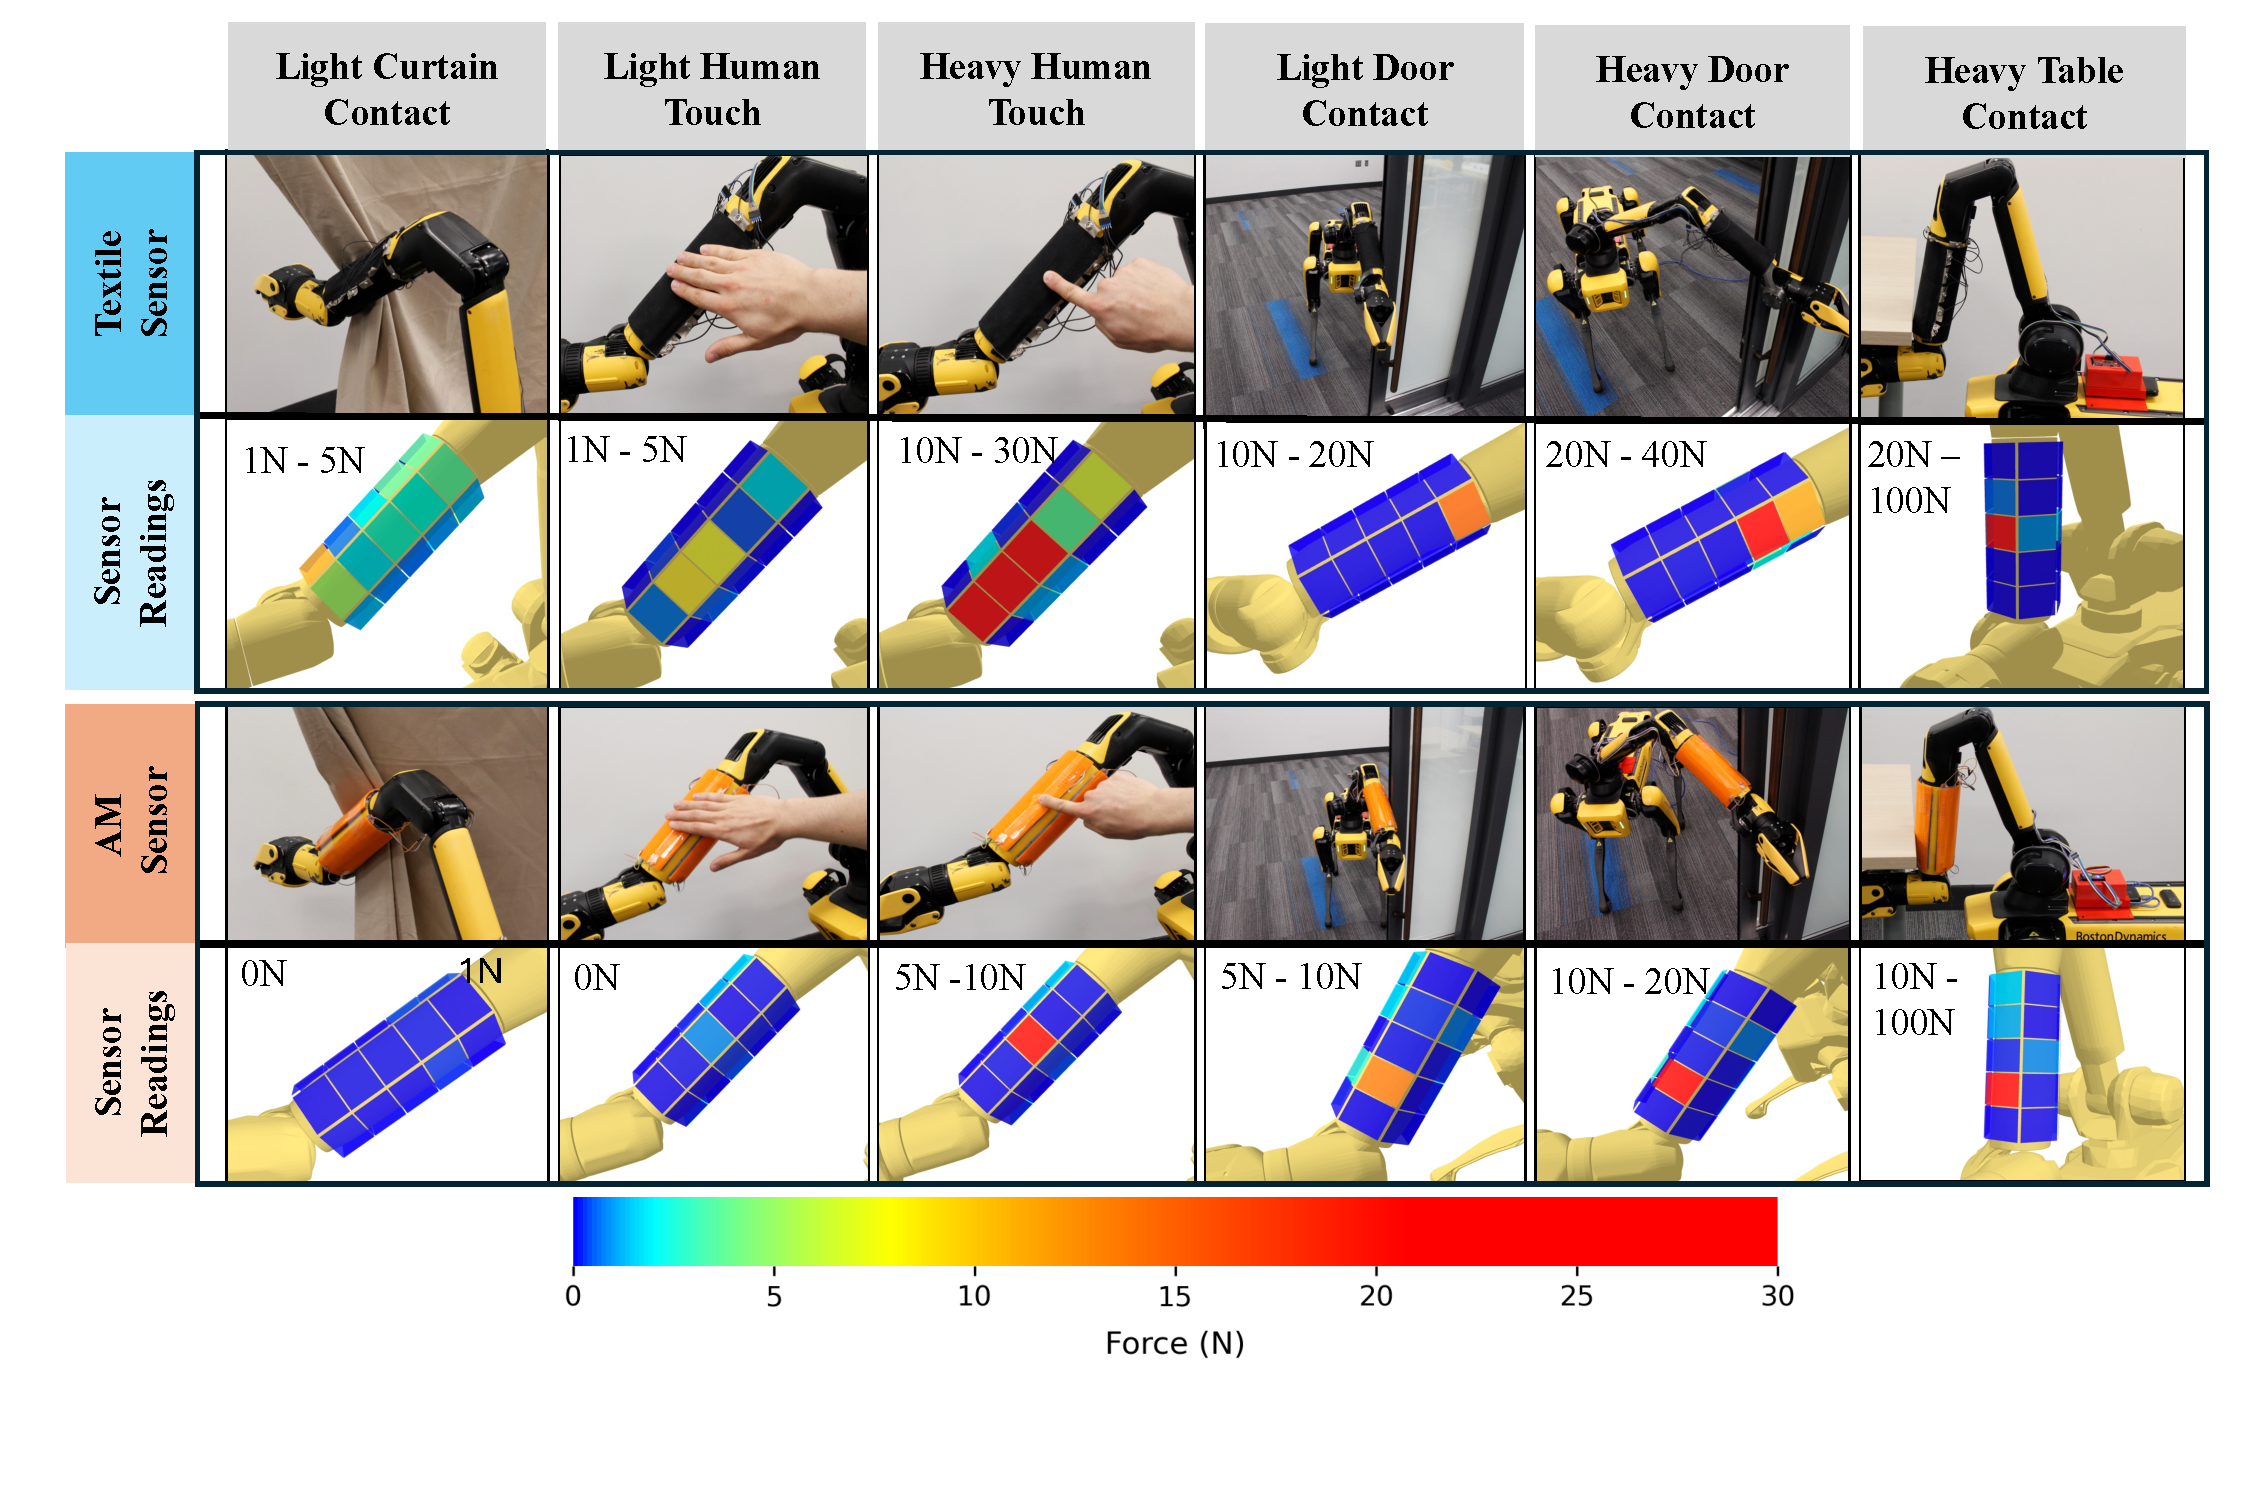
\includegraphics[width=0.90\linewidth,height=0.72\textheight,keepaspectratio]{Results_V6.pdf}

    \vspace{0.4em}
\end{frame}

\begin{frame}{Use Case 1: Contact Avoidance (Textile)}
    \centering
    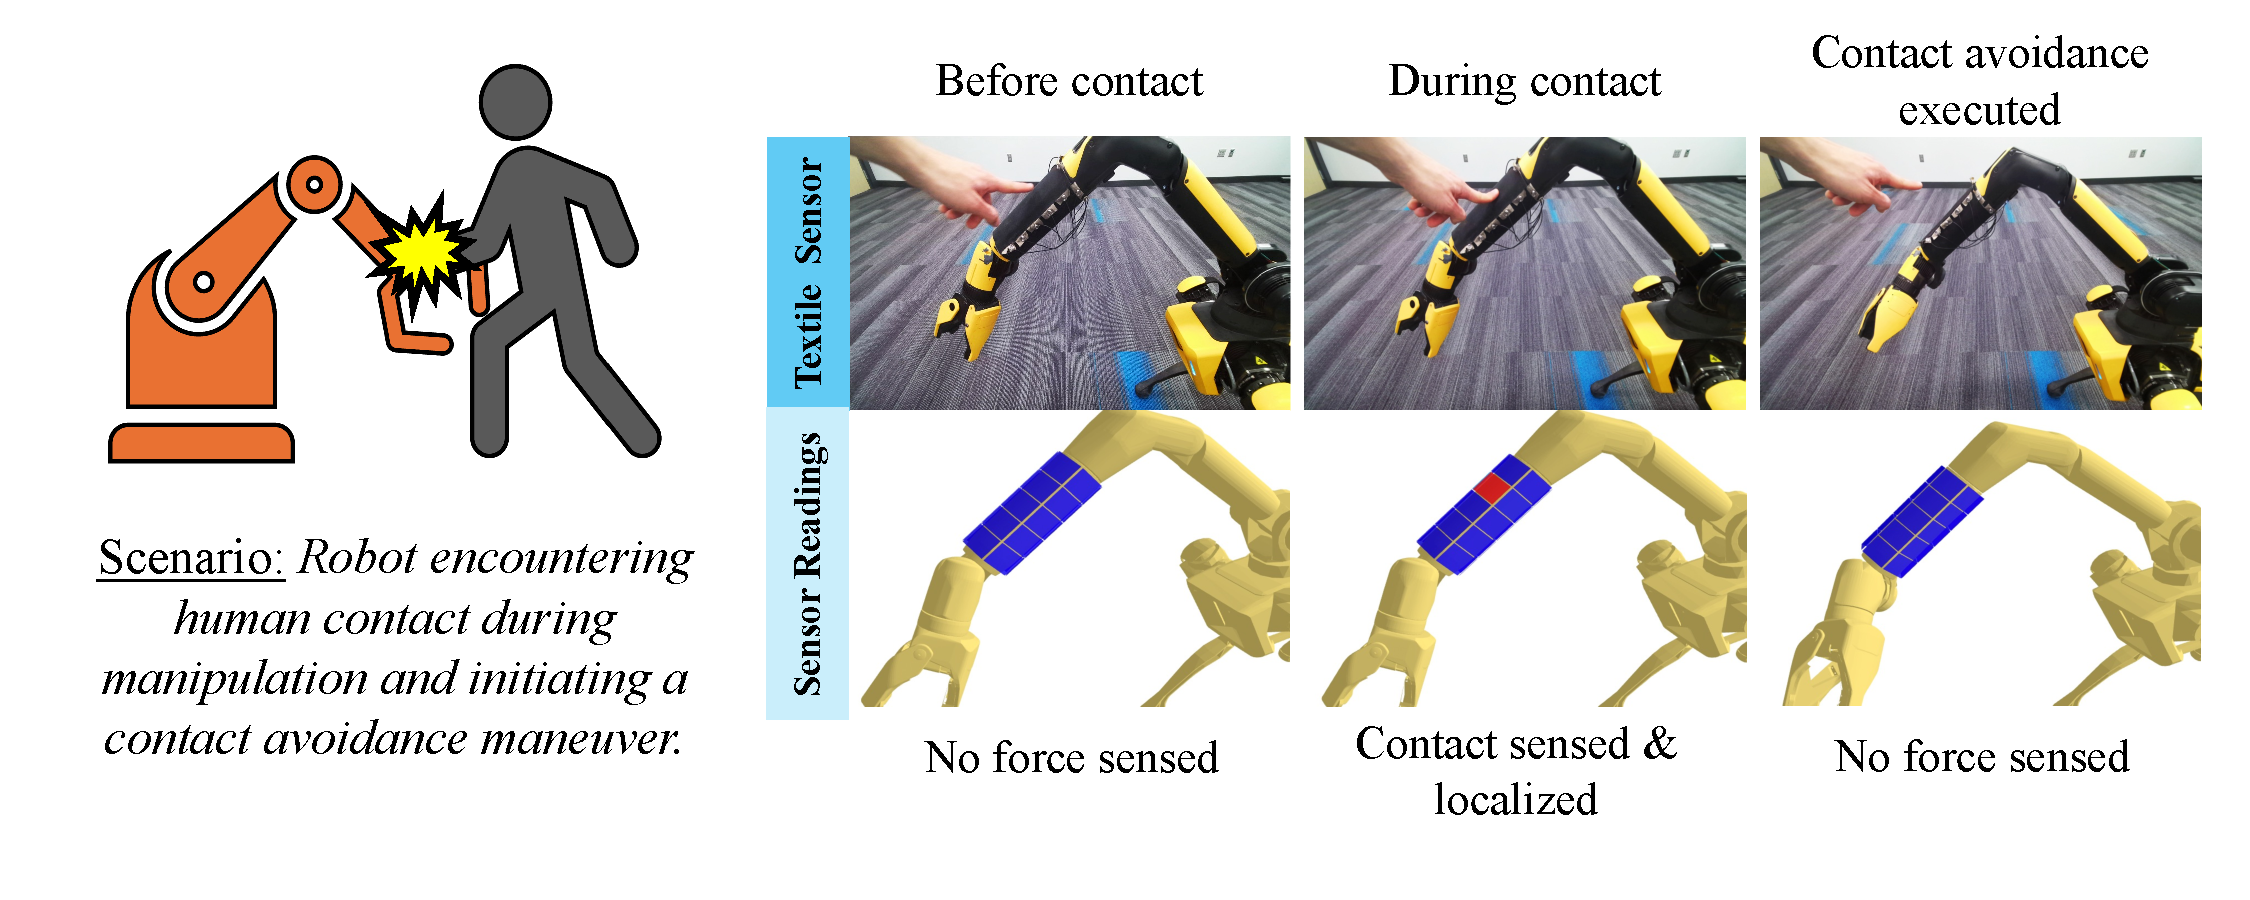
\includegraphics[width=0.92\linewidth,height=0.72\textheight,keepaspectratio]{Contact_Avoidance_V1.pdf}

    \vspace{0.4em}
\end{frame}

\begin{frame}{Use Case 2: Contact Embracing (AM)}
    \centering
    \includegraphics[width=0.92\linewidth,height=0.72\textheight,keepaspectratio]{FIg_Embrace_V4.pdf}

    \vspace{0.4em}
\end{frame}

\begin{frame}{Takeaways}
    \small
    \begin{itemize}
        \item Two low-cost ($<\$10$/link), complementary whole-arm tactile skin designs.
        \item Textile and AM variants cover distinct, practical force-interaction regimes.
        \item Figure-backed results show practical deployment for both avoidance and embracing contact.
    \end{itemize}

    \vspace{0.8em}
    \centering
    \Large Questions?
\end{frame}

\end{document}
